\section{Introduction}
\label{intro}

% \begin{table*}[t]
% \centering
% \begin{tabular}{cccc}
% \toprule
% \multicolumn{1}{c}{\bf{Map}} & \bf{Fold}  & \bf{FlatMap} & \bf{HashReduce} \\ \midrule
% \texttt{\footnotesize{Indices}}\vspace{-0.5mm} &
% \texttt{\footnotesize{Indices}}\vspace{-0.5mm} &
% \texttt{\footnotesize{ Indices}}\vspace{-0.5mm} &
% \texttt{\footnotesize{  Indices}}\vspace{-0.5mm} \\

% \belowbaseline[-25pt]{ 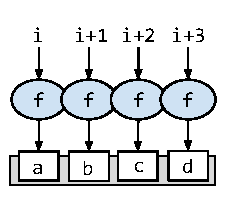
\includegraphics[width=2.5cm]{figs/Map.pdf}  }&
% \belowbaseline[-20pt]{ 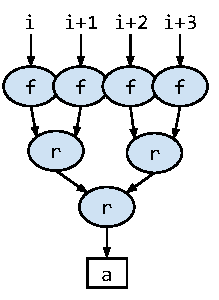
\includegraphics[width=2.5cm]{figs/Reduce.pdf}  }&
% \belowbaseline[-20pt]{ 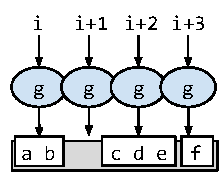
\includegraphics[width=2.5cm]{figs/FlatMap.pdf} }&
% \belowbaseline[-20pt]{ 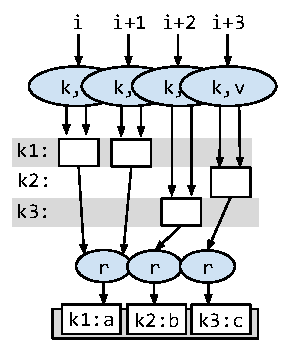
\includegraphics[height=3.4cm, width=3.24cm]{figs/HashReduce.pdf} }\\
% \bottomrule
% \end{tabular}
% %\vspace{-10pt}
% \caption{The parallel patterns in our programming model.}
% \vspace{-20pt}
% \label{t:patterns}
% \end{table*}


%\gist{Specialized hardware offers massive performance and energy benefits, but is expensive.}
In the search for higher performance and energy efficiency, computing
systems are steadily moving towards the use of specialized
accelerators~\cite{dadiannao, casper, q100, linqits, eyeriss, eie, LAP_TC12}. 
Accelerators implement customized data and control paths to
suit a domain of applications, thereby avoiding many of the overheads of
flexibility in general-purpose processors.  However, specialization in
the form of dedicated ASICs is expensive due to the high NRE costs for
design and fabrication, as well as the high deployment and iteration
times. This makes ASIC accelerators impractical for all but the most
ubiquitous applications.

%\gist{Spatial architectures: A Promising alternative. Designing a good accelerator architecture involves striking the right balance between
%flexibility, efficiency, and programmability.}
{\it Reconfigurable architectures} like FPGAs offset the high NRE
fabrication costs by providing flexible logic blocks in a statically
programmable interconnect to implement custom datapaths. 
In FPGAs, these custom datapaths are configurable at the bit level, allowing
users to prototype arbitrary digital logic and take advantage of architectural
support for arbitrary precision computation.
This flexibility has resulted in a number of successful commercial
FPGA-based accelerators deployed in data centers~\cite{catapult, catapultdnn, baidu}.   
However, flexibility comes at the cost of architectural inefficiencies.
Bit-level reconfigurability in computation and interconnect resources
comes with significant area and power overheads.
%\matt{difficult to parse this sentence ->} {\it
%Fine-grained reconfigurability} at the bit-level
%in compute and interconnect resources \emph{bit-level interconnects}
%introduces area and power overheads.
For example, over 60\% of the chip area and power in an FPGA is spent
in the programmable interconnect~\cite{fpgaSurvey, calhoun, bolsens, fpgaPower}. 
Long combinational paths through multiple logic elements
limit the maximum clock frequency at which an accelerator design can
operate. These inefficiencies have motivated the development of
coarse-grain reconfigurable architectures (CGRAs) with
word-level functional units that match the compute needs of most
accelerated applications. CGRAs provide dense compute resources,
%\matt{is "area density" a thing, or is it "chip area" or "compute density?"}
power efficiency, and clock frequencies up to an order of magnitude
higher than FPGAs. Modern commercial FPGA architectures such as Intel's Arria 10 and Stratix 10 device families have evolved to include
increasing numbers of coarse-grained blocks, including integer
multiply-accumulators (``DSPs''), floating point units, pipelined interconnect, and DRAM memory controllers.
The interconnect in these FPGAs, however, remains fine-grained to enable the devices to serve their original
purpose as prototyping fabrics for arbitrary digital logic.
%These advantages have motivated FPGA vendors to
%incorporate coarse-grained hardware blocks like DSPs and, most recently, floating point operators in their architectures.

%FPGAs have suffered from \emph{low-level programming models}, where logic
%synthesis tools typically expect designs to be specified in VHDL or Verilog.
%High-level FPGA compilers~\cite{vivadohls,legup, delite2maxj} alleviate only part of the problem,
%as tools are still required to perform place-and-route to produce a valid
%configuration bitstream satisfying all design constraints.  Bit-level place and route
%is time-consuming for large applications, leading to \emph{unreasonably long
%compile times} that hampers
%productivity~\cite{fpgaProgramming}.

\begin{table}[t]
\centering
\begin{tabular}{cccc}
\toprule
\bf{Map} & \bf{FlatMap} \\ \midrule
\texttt{\footnotesize{Indices}}\vspace{-0.5mm} &
\texttt{\footnotesize{Indices}}\vspace{-0.5mm} \\
\belowbaseline[-25pt]{ 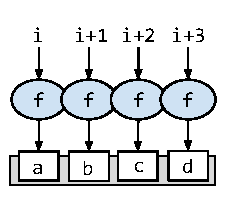
\includegraphics[width=2.5cm]{figs/Map.pdf}  }&
\belowbaseline[-20pt]{ 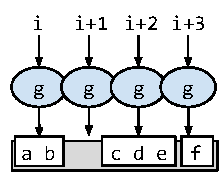
\includegraphics[width=2.5cm]{figs/FlatMap.pdf} } \\ \midrule

\bf{Fold} & \bf{HashReduce} \\ \midrule

\texttt{\footnotesize{ Indices}}\vspace{-0.5mm} &
\texttt{\footnotesize{  Indices}}\vspace{-0.5mm} \\
\belowbaseline[-20pt]{ 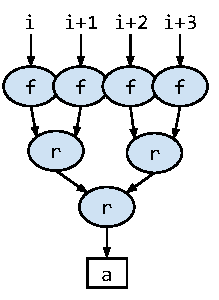
\includegraphics[width=2.5cm]{figs/Reduce.pdf}  } &
\belowbaseline[-20pt]{ 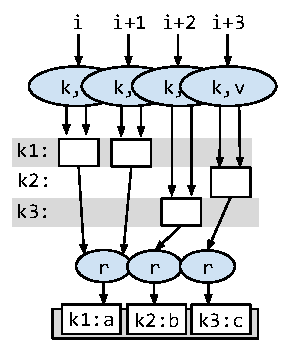
\includegraphics[height=3.4cm, width=3.24cm]{figs/HashReduce.pdf} }\\
\bottomrule
\end{tabular}

\caption{The parallel patterns in our programming model.}
\vspace{-20pt}
\label{t:patterns}
\end{table}


%\gist{Co-designing architecture and compiler is necessary to achieve
%the right balance}
Unfortunately, both FPGAs and previously proposed CGRAs are difficult
to use. Accelerator design typically involves low-level programming
models and long compilation times~\cite{fpgaVsAsic, fpgaSurvey,
  fpgaProgramming}. The heterogeneity of resources in most CGRAs and
in FPGAs with coarse-grain blocks adds further complications.
%\matt{I think the last
%sentence in the paragraph already says everything this sentence does}
%The goal of this work
%is to {\it develop a reconfigurable fabric that is both highly
%  efficient in terms of area, power, and performance and easy to use
%  in terms of programming and compilation complexity}.
A promising approach towards simplifying accelerator development is to
start with domain-specific languages that capture high-level parallel
patterns such as map, reduce, filter, and
flatmap~\cite{ecoop13sujeeth,pldi13halide}.  Parallel patterns have
been successfully used to simplify parallel programming and code
generation for a diverse set of parallel architectures including
multi-core chips~\cite{scala,haskell,delite-tecs14} and
GPUs~\cite{catanzaro11copperhead,micro14lee}.  Recent work has shown
that parallel patterns can also be used to generate optimized accelerators
for FPGAs from high-level languages~\cite{delite2maxj,george14fpl}.
In this work, we focus on developing a coarse-grain, reconfigurable
fabric with direct architectural support for parallel patterns which
is both highly efficient in terms of area, power, and performance and
easy to use in terms of programming and compilation complexity.

% May want to re-use some of the text below
% Our approach to designing a reconfigurable architecture is to
% simultaneously design the compilation flow and programming environment
% while considering application characteristics.  Applications amenable
% to hardware acceleration typically exhibit certain key characteristics
% such as parallelism at multiple levels of nesting and data
% locality. The architecture must be able to exploit these
% characteristics with the right set of reconfigurable primitives to
% achieve high execution efficiency.  The choice and granularity of
% reconfigurable primitives used in the architecture impacts its
% configuration interface, which, in turn, significantly impacts the
% complexity and efficiency of the compiler.  Reconfigurable
% architectures designed in isolation without considering application
% characteristics or compiler flows can end up being imbalanced, with
% either too much flexibility and associated compiler complexity, or too
% little flexibility by hardwiring the architecture to a narrow domain
% of operations. We therefore believe that the right balance between
% efficiency, flexibility, and programmability in reconfigurable
% architectures can be achieved by co-designing the architecture,
% compiler, and programming model.

% \gist { Introduce PCUs, PMUs (decide its name), three kinds of interconnect,
% memory address generators. Specifically: PCUs: SIMD Pipeline, reduction network,
% shift network; PMUs: On-chip address generation (reference decoupled access-execute?),
% scratchpad with various banking modes; Interconnect: Pipelined, with some compute
% capability that enables decentralized control scheme for hierarchical pipelines;
% address generators with coalescing to handle DRAM requests
% }
We introduce {\it Plasticine}, a new spatially reconfigurable
accelerator architecture optimized for efficient execution of parallel
patterns.  Plasticine is a two dimensional array of two kinds of coarse-grained reconfigurable units:
\emph{Pattern Compute Units} (PCUs) and \emph{Pattern Memory Units} (PMUs). 
Each PCU consists of a reconfigurable pipeline with multiple stages of SIMD functional units, with support
for cross-SIMD lane shifting and reduction. 
PMUs are composed of a banked scratchpad memory and dedicated addressing logic and address decoders.
These units communicate with each other through a pipelined \emph{static hybrid interconnect} with
separate bus-level and word-level data, and bit-level control networks. The
hierarchy in the Plasticine architecture simplifies compiler mapping and improves
execution efficiency. The compiler can map inner loop computation to one PCU 
such that most operands are transferred
directly between functional units without scratchpad accesses or
inter-PCU communication. The on-chip, banked scratchpads are
configurable to support streaming and double buffered accesses.
The off-chip memory controllers
support both streaming (burst) patterns and scatter/gather
accesses. Finally, the on-chip control logic is configurable to
support nested patterns.



% \christos{Need to edit below} In this paper, we introduce
% \emph{SPATIAL}, a new programming language and compiler for
% reconfigurable architectures, and \emph{Plasticine}, a new spatially
% reconfigurable accelerator architecture. SPATIAL provides a
% \emph{high-level programming interface} to specify applications using
% constructs that capture parallelism and data locality.  The SPATIAL
% compiler provides a \emph{fast, efficient compiler flow} from SPATIAL
% to Plasticine configurations. The compiler represents applications
% internally as a hierarchical dataflow graph, and provides an automated
% compilation flow performs a series of passes to optimize, schedule,
% map, and route the design onto Plasticine.\todo{ Need to make a
%   comment about the parallelism and locality extracted from Spatial
%   programs matches configuration parameters of Plastcinie so
%   compilation is easier and faster (no logic synthesis, no bit-level
%   palce and route)}
%\christos{This paragraphs describes what but not why. You
%  should be able to connect each feature but to requirements listed above}

% %\gist{Key Contributions}
% We make the following key contributions in this paper:
% \begin{itemize}
%   \item We describe \emph{Plasticine}, a reconfigurable architecture that provides
%     a flexible hardware substrate to efficiently accelerate a broad range applications
%     with different kinds of parallelism, memory access patterns, and data locality;
%   \item We describe \emph{SPATIAL}, a high-level programming language and compiler
%     that provides an automated flow from application to Plasticine configurations.
%   \item Evaluation - Performance, Perf/W, Compilation time
% \end{itemize}

% \christos{Think of reviewer 3 that asks ``why do I need one more of
%   these?'' This has to be clear in the intro. For example, why don't I
% point Spatial to one of the many CGRAs? What SPATIAL has that other
% dataflow languages don't have for specialized computing? etc. The
% easiest way to do this is a) justify early why the features in table 1
% are the important one (if nobody has all of them, this worth trying)
% and b) explain a little what is the link between SPATIAL and
% Plasticine (how the arch features help with fast compilation etc)
% because rigth now it is not obvious.}

We have implemented Plasticine in Chisel~\cite{chisel}, a Scala-based hardware definition
language.  We obtain area estimates after synthesizing the design using Synopsys Design Compiler,
and power numbers using simulation traces and PrimeTime.
Using VCS and DRAMSim2 for cycle-accurate simulation, we perform detailed evaluation of
the Plasticine architecture on a wide range of dense and sparse benchmarks in the domains of linear algebra, machine
learning, data analytics and graph analytics.

The rest of this paper is organized as follows: Section~\ref{patterns}
reviews the key concepts in parallel patterns and their hardware
implementation. Section~\ref{plasticine} introduces the Plasticine architecture and
explores key design tradeoffs. Section~\ref{evaluation} evaluates
the power and performance efficiency of Plasticine versus an FPGA.
Section~\ref{relatedWork} discusses related work. 



